%%%%%%%%%%%%%%%%%%%%%%%%%%%%%%%%%%%%%%%%%%%%%%%%%%%%%%%%%%%%%%%%%%%%%%
\section{\label{sec:GridUniverse}The Grid Universe}
%%%%%%%%%%%%%%%%%%%%%%%%%%%%%%%%%%%%%%%%%%%%%%%%%%%%%%%%%%%%%%%%%%%%%%

\index{HTCondor-C|(}

%%%%%%%%%%%%%%%%%%%%%%%%%%%%%%%%%%%%%%%%%%%%%%%%%%%%%%%%%%%%%%%%%%%%%%%%%%%
\subsection{\label{sec:HTCondor-C}HTCondor-C, The condor Grid Type }
%%%%%%%%%%%%%%%%%%%%%%%%%%%%%%%%%%%%%%%%%%%%%%%%%%%%%%%%%%%%%%%%%%%%%%%%%%%

\index{grid computing!HTCondor-C}
HTCondor-C allows jobs in one machine's job queue to
be moved to another machine's job queue.
These machines may be far removed from each other,
providing powerful grid computation mechanisms,
while requiring only HTCondor software and its configuration.

HTCondor-C is highly resistant to network disconnections and machine failures on both the submission and remote sides.
An expected usage
sets up Personal HTCondor on a laptop,
submits some jobs that are sent to an HTCondor pool,
waits until the jobs are staged on the pool,
then turns off the laptop.
When the laptop reconnects at a later time,
any results can be pulled back.

HTCondor-C scales gracefully when compared with HTCondor's flocking
mechanism.
The machine upon which jobs are submitted
maintains a single process and network connection to a remote machine,
without regard to the number
of jobs queued or running.

%%%%%%%%%%%%%%%%%%%%%%%%%%%%%%%%%%%%%%%%%%%%%%%%%%%%%%%%%%%%%%%%%%%%%%%%%%%
\subsubsection{\label{sec:HTCondor-C-Config}HTCondor-C Configuration}
%%%%%%%%%%%%%%%%%%%%%%%%%%%%%%%%%%%%%%%%%%%%%%%%%%%%%%%%%%%%%%%%%%%%%%%%%%%
\index{HTCondor-C!configuration}
There are two aspects to configuration to enable the
submission and execution of HTCondor-C jobs.
These two aspects correspond to the endpoints of the 
communication: there is the machine from which jobs are
submitted, and there is the remote machine upon which the
jobs are placed in the queue (executed).

Configuration of a machine from which jobs are submitted
requires a few extra configuration variables:

\footnotesize
\begin{verbatim}
CONDOR_GAHP=$(SBIN)/condor_c-gahp
C_GAHP_LOG=/tmp/CGAHPLog.$(USERNAME)
C_GAHP_WORKER_THREAD_LOG=/tmp/CGAHPWorkerLog.$(USERNAME)
\end{verbatim}
\normalsize

\index{HTCondor GAHP}
\index{GAHP (Grid ASCII Helper Protocol)}
The acronym GAHP stands for Grid ASCII Helper Protocol.
A GAHP server provides grid-related services for a
variety of underlying middle-ware systems.
The configuration variable \Macro{CONDOR\_GAHP}
gives a full path to the GAHP server utilized by HTCondor-C.
The configuration variable \Macro{C\_GAHP\_LOG} defines
the location of the log that the HTCondor GAHP server writes.
The log for the HTCondor GAHP is written as the user on whose
behalf it is running; thus the
\Macro{C\_GAHP\_LOG} configuration variable must point to a location the end
user can write to.

A submit machine must also have a \Condor{collector} daemon to which the
\Condor{schedd} daemon can submit a query.
The query is for the location (IP address and port)
of the intended remote machine's \Condor{schedd} daemon.
This facilitates communication between the two machines.
This \Condor{collector} does not need to be the same collector
that the local \Condor{schedd} daemon reports to.

The machine upon which jobs are executed 
must also be configured correctly.
This machine must be running a \Condor{schedd} daemon.
Unless specified explicitly in a submit file, 
\MacroNI{CONDOR\_HOST} must point to a 
\Condor{collector} daemon that it can write to,
and the machine upon which jobs are submitted can read from.
This facilitates communication between the two machines.

An important aspect of configuration is the security 
configuration relating to authentication.
HTCondor-C on the remote machine relies on an
authentication protocol to
know the identity of the user under which to run a job.
The following is a working example
of the security configuration for authentication.
This authentication method, CLAIMTOBE, 
trusts the identity claimed by a host or IP address.

\footnotesize
\begin{verbatim}
SEC_DEFAULT_NEGOTIATION = OPTIONAL
SEC_DEFAULT_AUTHENTICATION_METHODS = CLAIMTOBE
\end{verbatim}
\normalsize

Other working authentication methods are
GSI, SSL, KERBEROS, and FS.


%%%%%%%%%%%%%%%%%%%%%%%%%%%%%%%%%%%%%%%%%%%%%%%%%%%%%%%%%%%%%%%%%%%%%%%%%%%
\subsubsection{\label{sec:HTCondor-C-Submit}HTCondor-C Job Submission}
%%%%%%%%%%%%%%%%%%%%%%%%%%%%%%%%%%%%%%%%%%%%%%%%%%%%%%%%%%%%%%%%%%%%%%%%%%%
\index{HTCondor-C!job submission}
\index{universe!grid}
Job submission of HTCondor-C jobs is the same as for any HTCondor job.
The \SubmitCmd{universe} is \SubmitCmd{grid}.
\SubmitCmd{grid\_resource} specifies the remote \Condor{schedd} daemon to which
the job should be submitted, and its value consists of three fields.
The first field is the grid type, which is \SubmitCmd{condor}.
The second field is the name of the remote \Condor{schedd} daemon.
Its value is the
same as the \Condor{schedd} ClassAd attribute \Attr{Name} on the
remote machine.
The third field is the name of the remote pool's \Condor{collector}.
%and the \SubmitCmd{grid\_type} is \SubmitCmd{condor}. 
%The remote pool's job queue is defined and located by
%the submit description file command \SubmitCmd{remote\_schedd}.
%The value assigned for this command is the same as
%the \Condor{schedd} ClassAd attribute
%\Attr{Name} on the remote machine.
%The remote pool's \Condor{collector} is defined by the submit
%description file command \SubmitCmd{remote\_pool}.

The following represents a minimal submit description file for
a job.

\footnotesize
\begin{verbatim}
# minimal submit description file for an HTCondor-C job
universe = grid
executable = myjob
output = myoutput
error = myerror
log = mylog

grid_resource = condor joe@remotemachine.example.com remotecentralmanager.example.com
+remote_jobuniverse = 5
+remote_requirements = True
+remote_ShouldTransferFiles = "YES"
+remote_WhenToTransferOutput = "ON_EXIT"
queue
\end{verbatim}
\normalsize

The remote machine needs to understand the attributes of the job.
These are specified in the submit description file using the '+'
syntax, followed by the string \SubmitCmd{remote\_}.
At a minimum, this will be the job's \SubmitCmd{universe} and the job's
\SubmitCmd{requirements}.
It is likely that other attributes specific to the
job's \SubmitCmd{universe} (on the remote pool) will also be necessary.
Note that attributes set with '+' are inserted directly into
the job's ClassAd.  
Specify attributes as they 
must appear in the job's ClassAd, not the submit description file. 
For example,
the \SubmitCmd{universe} is specified using an integer assigned for
a job ClassAd \Attr{JobUniverse}.
Similarly, place quotation marks around string 
expressions.
As an example, a submit description file would ordinarily contain
\footnotesize
\begin{verbatim}
when_to_transfer_output = ON_EXIT
\end{verbatim}
\normalsize
This must appear in the HTCondor-C job submit description file as
\footnotesize
\begin{verbatim}
+remote_WhenToTransferOutput = "ON_EXIT"
\end{verbatim}
\normalsize

For convenience, the specific entries of 
\SubmitCmd{universe}, 
\SubmitCmd{remote\_grid\_resource}, 
\SubmitCmd{globus\_rsl}, and
\SubmitCmd{globus\_xml}
may be specified as \SubmitCmd{remote\_} commands
without the leading '+'. 
Instead of 
\footnotesize
\begin{verbatim}
+remote_universe = 5
\end{verbatim}
\normalsize

the submit description file command may appear as

\footnotesize
\begin{verbatim}
remote_universe = vanilla
\end{verbatim}
\normalsize

Similarly, the command
\footnotesize
\begin{verbatim}
+remote_gridresource = "condor schedd.example.com cm.example.com"
\end{verbatim}
\normalsize

may be given as

\footnotesize
\begin{verbatim}
remote_grid_resource = condor schedd.example.com cm.example.com
\end{verbatim}
\normalsize

% why we need +remote_ShouldTransferFiles, etc.
For the given example,
the job is to be run as a \SubmitCmd{vanilla} 
\SubmitCmd{universe} job at the remote pool.
The (remote pool's) \Condor{schedd} daemon is likely to
place its job queue data on a local disk 
and execute the job on another machine within the pool of machines.
This implies that the file systems for the resulting submit machine
(the machine specified by \SubmitCmd{remote\_schedd}) and
the execute machine (the machine that runs the job) will
\emph{not} be shared.
Thus,
the two inserted ClassAds
\footnotesize
\begin{verbatim}
+remote_ShouldTransferFiles = "YES"
+remote_WhenToTransferOutput = "ON_EXIT"
\end{verbatim}
\normalsize
are used to invoke HTCondor's file transfer mechanism. 



As HTCondor-C is a recent addition to HTCondor,
the universes, associated integer assignments,
and notes about the existence of functionality are given in 
Table~\ref{working-remote-universes}.
The note "untested" implies that
submissions under the given universe have not yet
been thoroughly tested.
They may already work.

% universes, and whether they work in HTCondor-C
% NEED TO UPDATE THIS TABLE FOR gt5 and cream
\begin{center}
\begin{table}[hbt]
\begin{tabular}{|l|l|l}
\textbf{Universe Name} & \textbf{Value} & \textbf{Notes}\\ \hline \hline
standard  & 1 & untested \\ \hline
vanilla   & 5 & works well \\ \hline
scheduler & 7 & works well \\ \hline
grid      & 9 & \\
 & grid\_resource is condor & works well \\
 & grid\_resource is cream & untested \\
 & grid\_resource is gt2  & works well \\
 & grid\_resource is gt5 & untested \\ 
 & grid\_resource is nordugrid & untested \\ 
 & grid\_resource is unicore & untested \\
 & grid\_resource is lsf & works well \\
 & grid\_resource is pbs & works well \\ \hline
java & 10 & untested \\ \hline
parallel & 11 & untested \\ \hline
local & 12 & works well \\ \hline
\end{tabular}
\caption{\label{working-remote-universes}Functionality of remote job universes with HTCondor-C}
\end{table}
\end{center}

For communication between \Condor{schedd} daemons on the submit
and remote machines,
the location of the remote \Condor{schedd} daemon is needed.
This information resides in the \Condor{collector} of the remote
machine's pool.
The third field of the \SubmitCmd{grid\_resource} command in the submit description file
says which \Condor{collector} should be queried for the remote \Condor{schedd}
daemon's location.
An example of this submit command is
\footnotesize
\begin{verbatim}
grid_resource = condor schedd.example.com machine1.example.com
\end{verbatim}
\normalsize
If the remote \Condor{collector} is not listening on the standard port
(9618), then the port it \emph{is} listening on needs to be specified:
\footnotesize
\begin{verbatim}
grid_resource = condor schedd.example.comd machine1.example.com:12345
\end{verbatim}
\normalsize

File transfer of a job's executable, \File{stdin}, \File{stdout}, and
\File{stderr} are automatic.
When other files need to be transferred using HTCondor's file transfer
mechanism
(see section~\ref{sec:file-transfer} on page~\pageref{sec:file-transfer}),
the mechanism is applied based on the resulting job universe on the
remote machine.


%%%%%%%%%%%%%%%%%%%%%%%%%%%%%%%%%%%%%%%%%%%%%%%%%%%%%%%%%%%%%%%%%%%%%%%%%%%
\subsubsection{\label{sec:HTCondor-C-CrossPlatform}
HTCondor-C Jobs Between Differing Platforms}
%%%%%%%%%%%%%%%%%%%%%%%%%%%%%%%%%%%%%%%%%%%%%%%%%%%%%%%%%%%%%%%%%%%%%%%%%%%

HTCondor-C jobs given to a remote machine running Windows
must specify the Windows domain of the remote machine.
This is accomplished by defining a ClassAd attribute for the job.
Where the Windows domain is different at the submit machine
from the remote machine, the submit description file 
defines the Windows domain of the remote machine with
\begin{verbatim}
  +remote_NTDomain = "DomainAtRemoteMachine"
\end{verbatim}

A Windows machine not part of a domain
defines the Windows domain as the machine name.

%%%%%%%%%%%%%%%%%%%%%%%%%%%%%%%%%%%%%%%%%%%%%%%%%%%%%%%%%%%%%%%%%%%%%%%%%%%
%\subsubsection{\label{sec:HTCondor-C-Hops}Multiple Hops for HTCondor-C Jobs}
%%%%%%%%%%%%%%%%%%%%%%%%%%%%%%%%%%%%%%%%%%%%%%%%%%%%%%%%%%%%%%%%%%%%%%%%%%%
%
% \Todo


\index{HTCondor-C|)}



\index{Condor-G|(}

%%%%%%%%%%%%%%%%%%%%%%%%%%%%%%%%%%%%%%%%%%%%%%%%%%%%%%%%%%%%%%%%%%%%%%%%%%%
\section{\label{sec:Condor-G}Condor-G}
%%%%%%%%%%%%%%%%%%%%%%%%%%%%%%%%%%%%%%%%%%%%%%%%%%%%%%%%%%%%%%%%%%%%%%%%%%%

Condor-G is a ``window to the grid.''
The function of Condor-G becomes clear
with a brief overview of the software that forms a Condor pool.
For this discussion, the software of a Condor pool is divided
into two parts.
The first part does job management.
It keeps track of a user's jobs.
You can ask the job management part of Condor to show
you the job queue, to submit new jobs to the system,
to put jobs on hold,
and to request information about jobs that have completed.
The other part of the Condor software
does resource management.
It keeps track of which machines are available to run jobs,
how the available machines should be utilized given all the users
who want to run jobs on them,
and when a machine is no longer available.
Condor-G works with grid resources, allowing users to
effectively submit jobs, manage jobs, and have jobs execute
on widely distributed machines.

A machine with the job management part installed
is called a submit machine.
A machine with the resource management part installed 
is called an execute machine.
Each machine may have one part or both.
Condor-G is the job management part of Condor.
\index{Condor-G!functionality}
Condor-G lets you submit jobs into a queue,
have a log detailing the life cycle of your jobs,
manage your input and output files,
along with everything else you expect from a job queuing system.

Condor-G is a program that manages both a queue of jobs
and the resources from one or more sites where those jobs can execute. 
For some of these jobs,
it communicates with these resources and transfers files
to and from these resources using Globus mechanisms.
(In particular, Condor-G uses the GRAM protocol for job submission,
and it runs a local GASS server for file transfers).

\Note This version of the manual has correct installation instructions
for Condor-G \VersionNotice, but other usage information has not
yet been updated.

%%%%%%%%%%%%%%%%%%%%%%%%%%%%%%%%%%%%%%%%%%%%%%%%%%%%%%%%%%%%%%%%%%%%%%%%%%%
\subsection{\label{sec:Globus-intro}Working with Globus}
%%%%%%%%%%%%%%%%%%%%%%%%%%%%%%%%%%%%%%%%%%%%%%%%%%%%%%%%%%%%%%%%%%%%%%%%%%%

The Globus software provides a well-defined set of protocols
that allow authentication, data transfer, and remote job submission.

Authentication is a mechanism by which an identity is verified.
Given proper authentication, authorization to use a resource
is required.
Authorization is a policy that determines who is allowed to do what. 


%%%%%%%%%%%%%%%%%%%%%%%%%%%%%%%%%%%%%%%%%%%%%%%%%%%%%%%%%%%%%%%%%%%%%%%%%%%
\subsubsection{\label{sec:Globus-Protocols}Globus Protocols}
%%%%%%%%%%%%%%%%%%%%%%%%%%%%%%%%%%%%%%%%%%%%%%%%%%%%%%%%%%%%%%%%%%%%%%%%%%%
Condor uses the following Globus protocols.
These protocols allow Condor to utilize grid machines for
the execution of jobs.
\begin{description}
\item[GSI]
The Globus Toolkit's Grid Security Infrastructure (GSI) provides essential
\index{Condor-G!GSI}
building blocks for other Grid protocols and Condor-G.
This authentication and authorization system
makes it possible to authenticate a user just once,
using public key infrastructure (PKI) mechanisms to verify
a user-supplied grid credential.
GSI then handles the mapping of the grid credential to the
diverse local credentials and authentication/authorization mechanisms that
apply at each site. 
\item[GRAM]
The Grid Resource Allocation and Management (GRAM) protocol supports remote
\index{Condor-G!GRAM}
submission of a computational request (for example, to run program P)
to a remote computational resource,
and it supports subsequent monitoring and control of the resulting
computation. 
\item[GASS]
The Globus Toolkit's Global Access to Secondary Storage (GASS) service provides
\index{Condor-G!GASS}
mechanisms for transferring data to and from a remote HTTP, FTP, or GASS server. 
Condor-G uses GASS to transfer the executable, stdin, stdout, and stderr
between the submission machine and the remote resource.
\end{description}

%%%%%%%%%%%%%%%%%%%%%%%%%%%%%%%%%%%%%%%%%%%%%%%%%%%%%%%%%%%%%%%%%%%%%%%%%%%
\subsubsection{\label{sec:Grid-Access}Accessing the Grid with Condor-G}
%%%%%%%%%%%%%%%%%%%%%%%%%%%%%%%%%%%%%%%%%%%%%%%%%%%%%%%%%%%%%%%%%%%%%%%%%%%

Condor-G allows the user to treat the Grid as a local resource,
and the same command-line tools perform basic job management such as:
\begin{itemize}
\item Submit a job, indicating an executable, input and output files,
and arguments
\item Query a job's status
\item Cancel a job
\item Be informed when events happen,
such as normal job termination or errors
\item Obtain access to detailed logs that provide a complete history of a job
\end{itemize}

These are features that Condor has provided for many years.
Condor-G extends this to the grid,
providing resource management 
while still providing fault tolerance and exactly-once execution 
semantics. 

\begin{figure}[hbt]
\centering
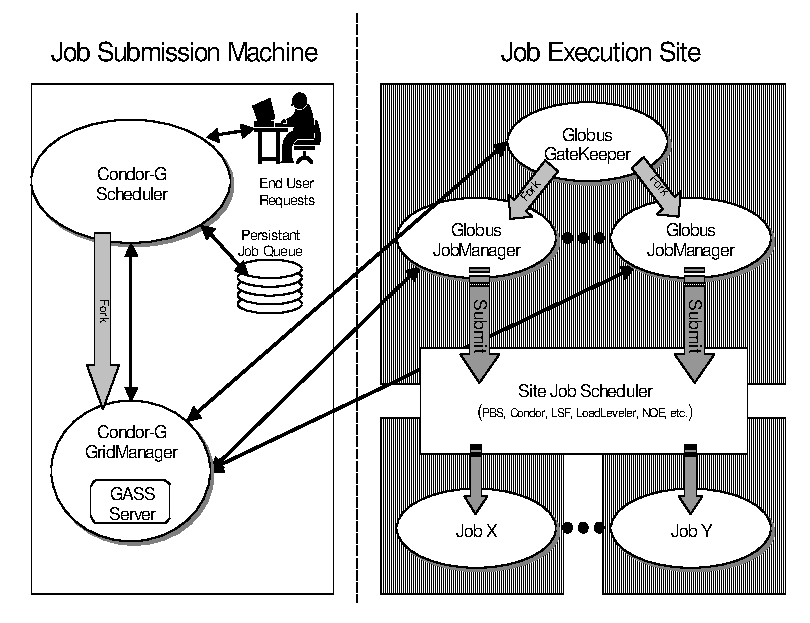
\includegraphics{grids/gfig1.eps}
\caption{\label{fig:condorg}Remote Execution by Condor-G on Globus managed resources}
\end{figure}

Figure~\ref{fig:condorg} shows how Condor-G interacts with Globus protocols.
Condor-G contains a GASS server, used to transfer the executable,
\File{stdin}, \File{stdout}, and \File{stderr} to and from
the remote job execution site.
Condor-G uses the GRAM protocol to contact the remote Globus Gatekeeper
and request that a new job manager be started.
GRAM is also used to monitor the job's progress.
Condor-G detects and intelligently handles cases
such as if the remote Globus resource crashes.

%%%%%%%%%%%%%%%%%%%%%%%%%%%%%%%%%%%%%%%%%%%%%%%%%%%%%%%%%%%%%%%%%%%%%%%%%%%
\subsection{\label{sec:Condor-G-Setup}Set Up of Condor-G}
%%%%%%%%%%%%%%%%%%%%%%%%%%%%%%%%%%%%%%%%%%%%%%%%%%%%%%%%%%%%%%%%%%%%%%%%%%%

%%%%%%%%%%%%%%%%%%%%%%%%%%%%%%%%%%%%%%%%%%%%%%%%%%%%%%%%%%%%%%%%%%%%%%%%%%%
\subsubsection{\label{sec:Condor-G-Install}Condor-G Installation}
%%%%%%%%%%%%%%%%%%%%%%%%%%%%%%%%%%%%%%%%%%%%%%%%%%%%%%%%%%%%%%%%%%%%%%%%%%%
\index{Condor-G!installation}
Condor-G is included in the standard Condor distribution.
Once Condor is obtained via download, installed, and configured,
(see
section~\ref{sec:install} on page~\pageref{sec:install})
there are two steps necessary before a globus universe job
can be submitted:

\begin{enumerate}

\item{Install Globus tools.}
Three ways are listed for obtaining the Globus tools:
   \begin{enumerate}
   \item{Globus}.
   From the web page at \URL{http://www.globus.org/}, follow links to the
   globus toolkit to get the resource management client bundle.
   \item{NMI}.
   From the web page at \URL{http://www.nsf-middleware.org/}, follow links
   to the NMI Release, and then to the Components, and finally to the
   Globus Toolkit. 
   \item{VDT}.
   From the web page at \URL{http://www.griphyn.org/vdt},
   follow the link to installing and setting up the Virtual Data Toolkit.
   \end{enumerate}

\item{Configure for Condor-G.}
If you installed Condor using the submit-only option, you will
need to add the following entries to your configuration file:
\begin{verbatim}
GRIDMANAGER             = $(SBIN)/condor_gridmanager
GAHP                    = $(SBIN)/gahp_server
MAX_GRIDMANAGER_LOG     = 64000
GRIDMANAGER_DEBUG       = D_COMMAND
GRIDMANAGER_LOG         = $(LOG)/GridLogs/GridmanagerLog.$(USERNAME)
GLIDEIN_SERVER_NAME     = gridftp.cs.wisc.edu
GLIDEIN_SERVER_DIR      = /p/condor/public/binaries/glidein
\end{verbatim}

If Condor-G is installed as root, the file
set by the configuration variable
\Macro{GRIDMANAGER\_LOG} must have world-write permission.
All of the parent directories for this file must
also have world-execute permission.
The Gridmanager runs as the user who submitted the job,
so the Gridmanager may not be able to write to the ordinary 
\MacroUNI{log} directory.
%The example configuration file sets the log file to be 
%\begin{verbatim}
%GRIDMANAGER_LOG = $(LOG)/GridLogs/GridmanagerLog.$(USERNAME) 
%\end{verbatim}
Use of the definition of \MacroNI{GRIDMANAGER\_LOG}
shown above will likely require the creation of
the directory \verb@$(LOG)/GridLogs@.
Permissions on this directory should be set
by running \Prog{chmod} using the value 1777. 

Another option is to locate the Gridmanager log files
somewhere else, like so:
\begin{verbatim}
GRIDMANAGER_LOG  = /tmp/GridmanagerLog.$(USERNAME)
\end{verbatim}

If you make any changes to the configuration file while
Condor is running, you will need to issue a \Condor{reconfigure}
command.

See section~\ref{sec:Configuring-Condor} on
page~\pageref{sec:Configuring-Condor} for
more information about configuration file entries.
See section~\ref{sec:Gridmanager-Config-File-Entries} on
page~\pageref{sec:Gridmanager-Config-File-Entries} for information
about  configuration file entries specific to the Condor-G
gridmanager.

\end{enumerate}

%%%%%%%%%%%%%%%%%%%%%%%%%%%%%%%%%%%%%%%%%%%%%%%%%%%%%%%
\subsubsection{\label{sec:Condor-G-Credentials}Credential Management}
%%%%%%%%%%%%%%%%%%%%%%%%%%%%%%%%%%%%%%%%%%%%%%%%%%%%%%%

(Reword this section to talk more about credential management and less
about specific config values. Also, probably move it out of the setup
section.)

Condor-G periodically checks for an updated proxy at
an interval given by the configuration variable
\AdAttr{GRIDMANAGER\_CHECKPROXY\_INTERVAL}.
The value is defined in terms of seconds.
For example, if you create a 12-hour proxy, and then
6 hours later re-run \Prog{grid-proxy-init},
Condor-G will check the proxy within
this time interval, and use the new proxy it finds there.
The default interval is 10 minutes.

Condor-G also knows when the proxy of each job will expire,
and if the proxy is not refreshed before
\AdAttr{GRIDMANAGER\_MINIMUM\_PROXY\_TIME}
seconds before the proxy expires,
the Condor-G grid manager daemon exits.
Since the grid manager daemon keeps track of all jobs
associated with a proxy, its tasks
(such as authentication, file transfer, job log maintainance)
will not occur.
So, if
\AdAttr{GRIDMANAGER\_MINIMUM\_PROXY\_TIME}
is 180, and the proxy is 3 minutes away from
expiring, Condor-G will attempt to safely shut down,
instead of simply losing
contact with the remote job because Condor-G is unable to
authenticate the remote job.
The default setting is 3 minutes (180 seconds).

%%%%%%%%%%%%%%%%%%%%%%%%%%%%%%%%%%%%%%%%%%%%%%%%%%%%%%%%%%%%%%%%%%%%%%%%%%%
\subsection{\label{sec:Using-Condor-G}Using the Globus Universe}
%%%%%%%%%%%%%%%%%%%%%%%%%%%%%%%%%%%%%%%%%%%%%%%%%%%%%%%%%%%%%%%%%%%%%%%%%%%

\index{universe!Globus}
This section contains what users need to know to 
run and manage jobs under the globus universe.

%%%%%%%%%%%%%%%%%%%%%%%%%%%%%%%%%%%%%%%%%%%%%%%%%%%%%%%%%%%%%%%%%%%%%%%%%%%
\subsubsection{\label{sec:Running-CondorG-Job}Running a Globus Universe Job}
%%%%%%%%%%%%%%%%%%%%%%%%%%%%%%%%%%%%%%%%%%%%%%%%%%%%%%%%%%%%%%%%%%%%%%%%%%%
\index{Condor-G!job submission}

Under Condor, successful job submission to the Globus universe requires
credentials.
An X.509 certificate is used to create a proxy,
and an account, authorization, or allocation to use a grid resource
is required.
For more information on proxies and certificates,
please consult the Alliance PKI pages at 

\URL{http://archive.ncsa.uiuc.edu/SCD/Alliance/GridSecurity/}

Before submitting a job to Condor under the Globus universe,
make sure you have your Grid 
credentials and have used \Prog{grid-proxy-init} to create a proxy.

A job is submitted for execution to Condor using the
\Condor{submit} command.
\index{Condor commands!condor\_submit}
\Condor{submit} takes as an argument
the name of a file called a submit description file.
\index{submit description file!globus universe}
The following sample submit description file runs a job on
the Origin2000 at NCSA.

\begin{verbatim}
executable = test
globusscheduler = modi4.ncsa.uiuc.edu/jobmanager
universe = globus
output = test.out
log = test.log
queue
\end{verbatim} 

The 
\AdAttr{executable}
for this example is
transferred from the local machine to the remote machine.
By default, Condor transfers the executable, as well as any
files specified by the \AdAttr{input} command.
Note that this executable must be compiled for the correct
intended platform.

The \AdAttr{globusscheduler} command is dependent on the
scheduling software available on remote resource.
This required command will change based on the Grid resource
intended for execution of the job.

All Condor-G jobs (intended for execution on Globus-controlled
resources) are submitted to the globus universe.
The \verb@universe = globus@ command is required
in the submit description file.

No input file is specified for this example job.
Any output (file specified by the \AdAttr{output})
or error (file specified by the \AdAttr{error})
is transferred 
from the remote machine to the local machine as it is produced.
This implies that these files may be incomplete in the case
where the executable does not finish running on the remote resource.
The job log file is maintained on the local machine.

To submit this job to Condor-G for execution on the
remote machine, use
\begin{verbatim}
condor_submit test.submit
\end{verbatim}
where \File{test.submit} is the name of the submit description file.

Example output from 
\Condor{q} for this submission looks like:
\footnotesize
\begin{verbatim}
% condor_q


-- Submitter: wireless48.cs.wisc.edu : <128.105.48.148:33012> : wireless48.cs.wi

 ID      OWNER         SUBMITTED     RUN_TIME ST PRI SIZE CMD
   7.0   epaulson     3/26 14:08   0+00:00:00 I  0   0.0  test

1 jobs; 1 idle, 0 running, 0 held
\end{verbatim}
\normalsize

After a short time, Globus accepts the job.
Again running \Condor{q} will now result in

\footnotesize
\begin{verbatim}
% condor_q


-- Submitter: wireless48.cs.wisc.edu : <128.105.48.148:33012> : wireless48.cs.wi

 ID      OWNER         SUBMITTED     RUN_TIME ST PRI SIZE CMD
   7.0   epaulson     3/26 14:08   0+00:01:15 R  0   0.0  test

1 jobs; 0 idle, 1 running, 0 held
\end{verbatim}
\normalsize

Then, very shortly after that, the queue will be empty again,
because the job has finished:

\footnotesize
\begin{verbatim}
% condor_q


-- Submitter: wireless48.cs.wisc.edu : <128.105.48.148:33012> : wireless48.cs.wi

 ID      OWNER            SUBMITTED     RUN_TIME ST PRI SIZE CMD

0 jobs; 0 idle, 0 running, 0 held
\end{verbatim}
\normalsize


A second example of a submit description file runs the Unix \Prog{ls}
program on a different Globus resource.

\footnotesize
\begin{verbatim}
executable = /bin/ls
Transfer_Executable = false
globusscheduler = vulture.cs.wisc.edu/jobmanager
universe = globus
output = ls-test.out
log = ls-test.log
queue
\end{verbatim} 
\normalsize

In this example, the executable (the binary) has been pre-staged.
The executable is on the remote machine, and it is not to
be transferred before execution.
Note that the required 
\AdAttr{globusscheduler} and \AdAttr{universe}
commands are present.
The command
\begin{verbatim}
Transfer_Executable = FALSE
\end{verbatim}
within the submit description file identifies the executable
as being pre-staged.
In this case, the 
\AdAttr{executable}
command gives the path to the executable on the remote machine.

A third example submits a Perl script to be run as a submitted
Condor job.
The Perl script both lists and sets
environment variables for a job.
Save the following Perl script with the name \File{env-test.pl},
to be used as a Condor job executable.

\begin{verbatim}
#!/usr/bin/env perl

foreach $key (sort keys(%ENV))
{
   print "$key = $ENV{$key}\n"
}

exit 0;
\end{verbatim}

Run the Unix command
\begin{verbatim}
chmod 755 env-test.pl
\end{verbatim}
to make the Perl script executable.

Now create the following submit description file
(Replace \File{biron.cs.wisc.edu/jobmanager} with a resource
you are authorized to use.):

\footnotesize
\begin{verbatim}
executable = env-test.pl
globusscheduler = biron.cs.wisc.edu/jobmanager
universe = globus
environment = foo=bar; zot=qux
output = env-test.out
log = env-test.log
queue
\end{verbatim}
\normalsize

When the job has completed, the output file \File{env-test.out}
should contain something like this:

\footnotesize
\begin{verbatim}
GLOBUS_GRAM_JOB_CONTACT = https://biron.cs.wisc.edu:36213/30905/1020633947/
GLOBUS_GRAM_MYJOB_CONTACT = URLx-nexus://biron.cs.wisc.edu:36214
GLOBUS_LOCATION = /usr/local/globus
GLOBUS_REMOTE_IO_URL = /home/epaulson/.globus/.gass_cache/globus_gass_cache_1020633948
HOME = /home/epaulson
LANG = en_US
LOGNAME = epaulson
X509_USER_PROXY = /home/epaulson/.globus/.gass_cache/globus_gass_cache_1020633951
foo = bar
zot = qux
\end{verbatim}
\normalsize


Of particular interest is the GLOBUS\_REMOTE\_IO\_URL environment variable.
Condor-G automatically starts up a GASS remote I/O
server on the submitting machine.
Because of the potential for either side of the connection to fail,
the URL for the server cannot be passed directly to the job.
Instead, it is put into a file, and the GLOBUS\_REMOTE\_IO\_URL
environment variable points to this file. 
Remote jobs can read this file and use the URL it contains
to access the remote GASS server running inside Condor-G.
If the location
of the GASS server changes (for example, if Condor-G restarts),
Condor-G will contact the Globus gatekeeper and update this file on
the machine where the job is running.
It is therefore important that all accesses to
the remote GASS server check this file for the latest location.

The following Perl script will use the GASS server in Condor-G
to copy input files to the execute machine.
(In our case, our remote job
is just going to count the number of lines in a file.
Hopefully, your job will be a bit more productive.)

\footnotesize
\begin{verbatim}
#!/usr/bin/env perl
use FileHandle;
use Cwd;

STDOUT->autoflush();
$gassUrl = `cat $ENV{GLOBUS_REMOTE_IO_URL}`;
chomp $gassUrl;

$ENV{LD_LIBRARY_PATH} = $ENV{GLOBUS_LOCATION}. "/lib";
$urlCopy = $ENV{GLOBUS_LOCATION}."/bin/globus-url-copy";

# globus-url-copy needs a full pathname
$pwd = getcwd();
print "$urlCopy $gassUrl/etc/hosts file://$pwd/temporary.hosts\n\n";
`$urlCopy $gassUrl/etc/hosts file://$pwd/temporary.hosts`;

open(file, "temporary.hosts");
while(<file>) {
print $_;
}

exit 0;
\end{verbatim}
\normalsize

Our submit file looks like this:

\footnotesize
\begin{verbatim}
executable = gass-example.pl
globusscheduler = biron.cs.wisc.edu/jobmanager
universe = globus
output = gass.out
log = gass.log
queue
\end{verbatim}
\normalsize

There are two optional submit description file commands
of note:
\AdAttr{x509userproxy} and
\AdAttr{globusrsl}.
The \AdAttr{x509userproxy} command specifies the path to
an X.509 proxy.
The command is of the form:
\begin{verbatim}
x509userproxy = /path/to/proxy
\end{verbatim}
If this optional command is not present in the submit description file,
then Condor-G checks the value of the environment variable
\Env{X509\_USER\_PROXY} for the location of the proxy.
If this environment variable is not present, then Condor-G
looks for the proxy in the file
\File{/tmp/x509up\_u0000},
where the trailing zeros in this file name are
replaced with the Unix user id.

The \AdAttr{globusrsl} command is used to add additional
attribute settings to a job's RSL string.
The format of the \AdAttr{globusrsl} command is
\begin{verbatim}
globusrsl = (name=value)(name=value)
\end{verbatim}
An example of this command in a submit description file
\begin{verbatim}
globusrsl = (project=Test_Project)
\end{verbatim}
This example's attribute name for the additional RSL is
\verb@project@, and the value assigned is \verb@Test_Project@.

%%%%%%%%%%%%%%%%%%%%%%%%%%%%%%%%%%%%%%%%%%%%%%%%%%%%%%%%%%%%%%%%%%%%%%%%%%%
\subsubsection{\label{sec:Condor-G-Limits}Limitations of Condor-G}
%%%%%%%%%%%%%%%%%%%%%%%%%%%%%%%%%%%%%%%%%%%%%%%%%%%%%%%%%%%%%%%%%%%%%%%%%%%
% This subsubsection used to reside in the file limitations.tex.
\index{Condor-G!limitations}
Submitting jobs to run under the globus universe has not yet
been perfected.
The following is a list of known limitations:

\begin{enumerate}
\item{No checkpoints.}
\item{No matchmaking.}
\item{File transfer is limited.}
There are no file transfer mechanisms for files other
than the executable, \File{stdin}, \File{stdout}, and \File{stderr}.
\item{No job exit codes.}
Job exit codes are not available.
\item{Limited platform availability.}
Condor-G is only available on Linux, Solaris,
Digital UNIX, and IRIX.
HP-UX support will hopefully be available later.
\end{enumerate}

%%%%%%%%%%%%%%%%%%%%%%%%%%%%%%%%%%%%%%%%%%%%%%%%%%
\subsection{\label{sec:Condor-G-Matchmaking}Condor-G-Matchmaking}
%%%%%%%%%%%%%%%%%%%%%%%%%%%%%%%%%%%%%%%%%%%%%%%%%%
\index{universe!Globus}
\index{Globus}
\index{matchmaking!on the Grid}
\index{grid computing!matchmaking}

In it simplest usage, Condor-G allows users to specify the single
grid site they wish to submit their job to.
Often this is sufficient: perhaps a user knows exactly which
grid site they wish to use,
or a higher-level resource broker
(such as the European Data Grid's resource broker)
has decided which grid site should be used.
But when users have a variety of sites to choose from and there
is no other resource broker to make the decision, Condor-G can use
matchmaking to decide which grid site a job should run on. 

Please note that Condor-G's matchmaking ability is relatively
new. Work is being done to improve it and make it easier to use. For
now, please expect some rough edges. 

Condor-G uses the same matchmaking mechanism that Condor uses: the
\Condor{collector} and \Condor{negotiator} daemons, which are described in
Section~\ref{sec:Condor-Daemons}. 

Two changes are required to use Condor-G's matchmaking.
First,
advertise grid sites that are available so that they are
known and considered during the matchmaking process.
This is accomplished by writing ClassAd attributes and
using \Condor{advertise} to place the attributes into the
ClassAd used in matchmaking.
The second change is to the
submit description file.
This file needs to specify requirements that describe what
type of grid site can be used, instead of identifying a specific grid site.

% Karen had editted to this point.

%%%%%%%%%%%%%%%%%%%%%%%%%%%%%%%%%%%%%%%%%%%%%%%%%%
\subsubsection{Advertising grid sites to Condor-G}
%%%%%%%%%%%%%%%%%%%%%%%%%%%%%%%%%%%%%%%%%%%%%%%%%%

Each grid site that is available for matching purposes needs to be
advertised to the \Condor{collector}. Normally in Condor this is done
with the \Condor{startd} daemon, and you do not normally need to be
aware of the contents of this advertisement. Currently, there is no
equivalent to the \Condor{startd} daemon for advertising grid sites,
so you need have a deeper understanding. 

To properly advertise a grid site, a ClassAd need to be sent
periodically to the \Condor{collector}. A ClassAd is a list of
attributes and values that describe a job, a machine, or a grid
site. ClassAds are briefly described in
Section~\ref{sec:matchmaking-with-classads} and some of the common
attributes of machine ClassAds are described in
Section~\ref{user-man-machad}.

When you advertise a grid site, it looks very similar to a ClassAd for
a machine. In fact, the \Condor{collector} will believe it is a
machine, but with a different set of attributes. 

To advertise a grid site, you first need to describe the site in a
file. Here is a sample ClassAd that describes a grid site:

\footnotesize
\begin{verbatim}
# This is a comment
MyType                = "Machine"
TargetType            = "Job"
Name                  = "Example1_Gatekeeper"
gatekeeper_url        = "grid.example.com/jobmanager"
Requirements          = (CurMatches < 10) && (TARGET.JobUniverse == 9)
Rank                  = 0.000000
CurrentRank           = 0.000000
WantAdRevaluate       = True
UpdateSequenceNumber  = 4
CurMatches            = 0
\end{verbatim}
\normalsize

Let's look at each line:

\begin{verbatim}
# This is a comment
\end{verbatim}

Your file can have comments that begin with the hash mark (\#). 

\begin{verbatim}
MyType                = "Machine"
\end{verbatim}

Your grid site is pretending to be a single machine, for the purpose
of matchmaking. \Attr{MyType} is an attribute that the \Condor{negotiator}
daemon
will expect to be a string. Strings must be surrounded by double-quote
marks, as in this example. You may have surprising, unintuitive errors
if they are not quoted. You will always want \Attr{MyType} to be
``Machine''. 

\begin{verbatim}
TargetType            = "Job"
\end{verbatim}

This is an attribute that says the grid site (machine) wants to be
matched with a job. Leave this as it is. 


\footnotesize
\begin{verbatim}
Name                  = "Example1_Gatekeeper"
\end{verbatim}
\normalsize

You will want a unique name for each grid site. Any name is fine, as long as
it is quoted.

\footnotesize
\begin{verbatim}
gatekeeper_url        = "grid.example.com/jobmanager"
\end{verbatim}
\normalsize

This is the Globus gatekeeper contact string for your grid site. It is
probably a machine name followed by a slash followed by the name of
the jobmanager. If you have different job managers, you can only
specify one per ClassAd. 

\begin{verbatim}
UpdateSequenceNumber  = 4
\end{verbatim}

UpdateSequenceNumber is a positive number that must increase each time
you advertise a grid site. Normally you advertise your grid site
every five minutes. The \Condor{collector} daemon will discard a grid site's
ClassAd after 15 minutes if there have been no updates. A good number
to set this to is the current time in seconds (the epoch, as given by
the C \Procedure{time} function call), but if you are worried about your clock
running backward, you can set it to whatever you like. If ClassAds are
received with a sequence number older than the last ClassAd, they are
ignored. 

\begin{verbatim}
CurMatches            = 0
\end{verbatim}

This number is incremented each time a match is made for this grid
site. Unlike a normal machine ClassAd that can only be matched against
once, grid site advertisements can be matched against many time. 

You will probably want to set this number to be the number of grid
jobs that you have running on your site, and keep it updated each time
you submit a new ClassAd. If you do not specify CurMatches, Condor
will assume it is 0.

Condor will increment this number every time it makes a match against
a grid site.

\footnotesize
\begin{verbatim}
Requirements          = (CurMatches < 10) && (TARGET.JobUniverse == 9)
\end{verbatim}
\normalsize

These are the requirements that the grid site insists must be true
before it will accept a job. These could refer to features of the
job's ClassAd. In this case, we will take any globus-universe job, as
long we have less than 10 matches currently. This will ensure that
Condor-G will only run 10 jobs at your site---assuming that you keep
CurMatches up to date when jobs finish. Of course, you can edit this
statement to have different requirements. For example, if you want to
accept all jobs, you can have \ShortExpr{Requirements = True}.

\footnotesize
\begin{verbatim}
Rank                  = 0.000000
CurrentRank           = 0.000000
\end{verbatim}
\normalsize

This is a numerical ranking that will be assigned to a job. Right now
it is not used, but should be set to 0. 

\begin{verbatim}
WantAdRevaluate       = True
\end{verbatim}

The \Attr{WantAdRevaluate} attribute distinguishes grid site
ClassAds from normal machine ClassAds and allows multiple matches to
be made against a single site. It should be in your ad and should be
true. Note that True is not in quotes, and it should not be.

You can add other attributes to your ClassAd, to make it easy for a
job to decide which grid site it wants to use. For instance, if you
have pre-installed the Bamboozle software environment on your grid
site, you could advertise, \ShortExpr{HaveBamboozle = True} and
\ShortExpr{BamboozleVersion = 10}. Jobs can require a grid site that has
Bamboozle installed by extending their requirements with
\ShortExpr{HaveBamboozle == True}. (Note the double equal sign in the
requirements.) 

As an aside, we recommend that jobs that need specific applications
should bring them with them instead of relying on having them
pre-installed at a Grid site. You will have more reliable execution if
you do. 

Once you have a file that describes your site, you need to send it to
the \Condor{collector} daemon. For this, use \Condor{advertise}.
We recommend that you write a script to create the file
containing the ClassAd, then run the script every five minutes with
\Prog{cron}. The script should probably update the \Attr{CurMatches}
variable, if you
want to restrict the number of grid jobs that can be submitted at one
time. 

For \Condor{advertise}, specify \Arg{UPDATE\_STARTD\_AD} for
the update command. For example, if your ClassAd is specified in a
file named \File{grid-ad} you would do:

\footnotesize
\begin{verbatim}
    condor_advertise UPDATE_STARTD_AD grid-ad
\end{verbatim}
\normalsize

\Condor{advertise} usually uses UDP to transmit your ClassAd. In
wide-area networks, this may be insufficient. You can use TCP by
specifying the \Opt{-tcp} option. 

%%%%%%%%%%%%%%%%%%%%%%%%%%%%%%%%%%%%%%%%%%%%%%%%%%
\subsubsection{Submitting Condor-G jobs that use matchmaking}
%%%%%%%%%%%%%%%%%%%%%%%%%%%%%%%%%%%%%%%%%%%%%%%%%%

Submitting a job to Condor-G that requires matchmaking is
straightforward. Instead of specifying a particular scheduler with
globussheduler like this:

\footnotesize
\begin{verbatim}
globusscheduler = grid.example.com/jobmanager
\end{verbatim}
\normalsize

you instead specify requirements and tell Condor-G where to find the
gatekeeper URL in the grid site ClassAd:

\footnotesize
\begin{verbatim}
globusscheduler = $$(gatekeeper_url)
requirements    = TARGET.gatekeeper_url =!= UNDEFINED
\end{verbatim}
\normalsize

This will allow to run at any grid site, and will extract the
gatekeeper\_url attribute from the ClassAd. There is no magic meaning
behind gatekeeper\_url---you could use GatekeeperContactString if you
desired, as long as it is the same in both the job description and the
grid site ClassAd. 

The requirements specified here are a bit simple. Perhaps you only
want to run at a site that has the Bamboozle software installed, and
the sites that have it installed specify ``HaveBamboozle = True'', as
described above. A complete job description may look like this:

\footnotesize
\begin{verbatim}
universe        = globus
executable      = analyze_bamboozle_data
output          = aaa.$(Cluster).out
error           = aaa.$(Cluster).err
log             = aaa.log
globusscheduler = $$(gatekeeper_url)
requirements    = (HaveBamboozle == True) && (TARGET.gatekeeper_url =!= UNDEFINED)
leave_in_queue  = jobstatus == 4
queue
\end{verbatim}
\normalsize

%%%%%%%%%%%%%%%%%%%%%%%%%%%%%%%%%%%%%%%%%%%%%%%%%%
\subsubsection{Advanced usage}
%%%%%%%%%%%%%%%%%%%%%%%%%%%%%%%%%%%%%%%%%%%%%%%%%%

What if a job fails to run at a grid site due to an error? It will be
returned to the queue, and Condor will attempt to match it and
re-run it at another site. Condor isn't very clever about avoiding
sites that may be bad, but you can give it some assistance. Let's say
that you want to avoid running at the last grid site you ran at. You
could add this to your job description:

\footnotesize
\begin{verbatim}
match_list_length = 1
Rank              = TARGET.Name != LastMatchName0
\end{verbatim}
\normalsize

This will prefer to run at a grid site that was not just tried, but it
will allow the job to be run there if there is no other option. 

When you specify match\_list\_length, you provide an integer N, and
Condor will keep track of the last N matches. The oldest match will be
LastMatchName0, and next oldest will be LastMatchName1, and so on. (See
the \Condor{submit} manual page for more details.) The Rank expression
allows you to specify a numerical ranking for different matches. When
combined with match\_list\_length, you can prefer to avoid sites that
you have already run at. 

In addition, \Condor{submit} has two options to help you control
Condor-G job resubmissions and rematching.  See globus\_resubmit and
globus\_rematch in the \Condor{submit} manual page. These options are
independent of match\_list\_length.

There are some new attributes that will be added to the Job ClassAd,
and may be useful to you when you write your rank, requirements,
globus\_resubmit or globus\_rematch option. Please refer to
Section~\ref{user-man-jobad} and read about the following option:

\begin{itemize}
\item NumJobMatches
\item NumGlobusSubmits
\item NumSystemHolds
\item HoldReason
\item ReleaseReason
\item EnteredCurrentStatus
\item LastMatchTime
\item LastRejMatchTime
\item LastRejMatchReason
\end{itemize}

If you are concerned about unknown or malicious grid sites reporting
to your \Condor{collector}, you should use Condor's security options,
documented in Section~\ref{sec:Security}.

%%%%%%%%%%%%%%%%%%%%%%%%%%%%%%%%%%%%%%%%%%%%%%%%%%
\subsubsection{\label{sec:HTCondor-G-GridMonitor}The Grid Monitor}
%%%%%%%%%%%%%%%%%%%%%%%%%%%%%%%%%%%%%%%%%%%%%%%%%%
\index{Grid Monitor}
\index{grid computing!Grid Monitor}
\index{scalability!using the Grid Monitor}

HTCondor's Grid Monitor is designed to improve the scalability of
machines running the Globus Toolkit's GRAM2 gatekeeper.
Normally, this service runs a jobmanager process for 
every job submitted to the gatekeeper.
This includes both currently running jobs and jobs waiting in the queue.
Each jobmanager runs a Perl script at
frequent intervals (every 10 seconds) to poll the state of
its job in the local batch system.
For example, with 400 jobs submitted to a gatekeeper,
there will be 400 jobmanagers running,
each regularly starting a Perl script.
When a large number of jobs
have been submitted to a single gatekeeper,
this frequent polling can heavily load the gatekeeper.
When the gatekeeper is under heavy load,
the system can become non-responsive, and a variety of problems can occur.

HTCondor's Grid Monitor temporarily replaces these jobmanagers.
It is named the Grid Monitor, because it replaces the monitoring
(polling) duties previously done by jobmanagers.
When the Grid Monitor runs,
HTCondor attempts to start a single
process to poll all of a user's jobs at a given gatekeeper.
While a job is waiting in the queue, but not yet running,
HTCondor shuts down the associated jobmanager,
and instead relies on the Grid Monitor to report changes in status.
The jobmanager started to add the job to the remote
batch system queue is shut down.
The jobmanager restarts when the job begins running.

The Grid Monitor requires that the gatekeeper support the fork
jobmanager with the name \Prog{jobmanager-fork}.
If the gatekeeper does not support the fork jobmanager,
the Grid Monitor will not be used for that site.
The \Condor{gridmanager} log file reports any problems
using the Grid Monitor.

The Grid Monitor is enabled by default,
and the
configuration macro \Macro{GRID\_MONITOR} identifies
the location of the executable.


%%%%%%%%%%%%%%%%%%%%%%%%%%%%%%%%%%%%%%%%%%%%%%%%%%
\section{\label{sec:Glidein}Glidein}
%%%%%%%%%%%%%%%%%%%%%%%%%%%%%%%%%%%%%%%%%%%%%%%%%%
\index{universe!grid}
\index{HTCondor commands!condor\_glidein}
\index{glidein}
\index{grid computing!glidein}

Glidein is a mechanism by which one or more grid resources (remote machines)
temporarily join a local HTCondor pool. 
The program \Condor{glidein} is used to add a machine
to an HTCondor pool.
During the period of time when the added resource is
part of the local pool, the resource is visible 
to users of the pool.
But, by default, the resource is only available for
use by the user
that added the resource to the pool.

After glidein, the user may submit jobs for execution on the
added resource the same way that all HTCondor jobs are submitted.
To force a submitted job to run on the added resource, the
submit description file could contain a requirement that the job run 
specifically on the added resource.


%%%%%%%%%%%%%%%%%%%%%%%%%%%%%%%%%%%%%%%%%%%%%%%%%%
\subsection{What \Condor{glidein} Does}
%%%%%%%%%%%%%%%%%%%%%%%%%%%%%%%%%%%%%%%%%%%%%%%%%%

\Condor{glidein} works by installing and executing
necessary HTCondor daemons and configuration on the remote resource,
such that the resource reports to and joins the local pool.
\Condor{glidein} accomplishes two separate tasks towards
having a remote grid resource join the local HTCondor pool.
They are the set up task and the execution task.

The set up task generates necessary 
configuration files and locates proper platform-dependent
binaries for the HTCondor daemons.
A script is also generated that can be used during
the execution task to invoke the proper HTCondor daemons.
These files are copied to the remote resource as necessary.
The configuration variable \Macro{GLIDEIN\_SERVER\_URLS}
defines a list of locations from which the necessary
binaries are obtained.
Default values cause binaries to be downloaded from the 
UW site.
See 
section~\ref{param:GlideinServerURLS} 
on page~\pageref{param:GlideinServerURLS}
for a full definition of this configuration variable.

When the files are correctly in place,
the execution task starts the HTCondor daemons.
\Condor{glidein} does this by submitting an HTCondor job
to run under the grid universe.
The job runs the \Condor{master} on the remote grid resource.
The \Condor{master} invokes other daemons, which contact
the local pool's \Condor{collector} to join the pool.
The HTCondor daemons exit gracefully when no jobs run on the daemons for a
preset period of time.

Here is an example of how a glidein resource appears, similar to how
any other machine appears.  The name has a
slightly different form, in order to handle the possibility of
multiple instances of glidein daemons inhabiting a multi-processor
machine.

\footnotesize
\begin{verbatim}
% condor_status | grep denal
7591386@denal LINUX       INTEL  Unclaimed  Idle       3.700  24064  0+00:06:35

\end{verbatim}
\normalsize

%%%%%%%%%%%%%%%%%%%%%%%%%%%%%%%%%%%%%%%%%%%%%%%%%%
\subsection{Configuration Requirements in the Local Pool}
%%%%%%%%%%%%%%%%%%%%%%%%%%%%%%%%%%%%%%%%%%%%%%%%%%
\index{configuration!for glidein}
\index{glidein!configuration}

As remote grid resources join the local pool,
these resources must report to the local pool's \Condor{collector} daemon.
Security demands that the local pool's \Condor{collector} 
list all hosts from which they will accept communication.
Therefore, all remote grid resources accepted for glidein
must be given
\Macro{HOSTALLOW\_WRITE} permission.
An expected way to do this is to modify the empty variable
(within the sample configuration file)
\MacroNI{GLIDEIN\_SITES} to list all remote grid resources
accepted for glidein.
The list is a space or comma separated list of hosts.
This list is then given the proper permissions by an additional
redefinition of the \MacroNI{HOSTALLOW\_WRITE} configuration variable,
to also include the list of hosts
as in the following example.

\footnotesize
\begin{verbatim}
GLIDEIN_SITES = A.example.com, B.example.com, C.example.com
HOSTALLOW_WRITE = $(HOSTALLOW_WRITE) $(GLIDEIN_SITES)
\end{verbatim}
\normalsize
Recall that for configuration file changes to take effect,
\Condor{reconfig} must be run.

If this configuration change to the security settings on
the local HTCondor pool cannot be made,
an additional HTCondor pool that utilizes
personal HTCondor may be defined.
The single machine pool
may coexist with other instances of HTCondor.
\Condor{glidein} is executed to have the remote grid
resources join this personal HTCondor pool.

%%%%%%%%%%%%%%%%%%%%%%%%%%%%%%%%%%%%%%%%%%%%%%%%%%
\subsection{Running Jobs on the Remote Grid Resource After Glidein }
%%%%%%%%%%%%%%%%%%%%%%%%%%%%%%%%%%%%%%%%%%%%%%%%%%

Once the Globus resource has been added to the local HTCondor
pool with \Condor{glidein},
job(s) may be submitted.
To force a job to run on the Globus resource,
specify that Globus resource as a machine requirement
in the submit description file. 
Here is an example from within the submit description file
that forces submission to the Globus resource denali.mcs.anl.gov:
\begin{verbatim}
      requirements = ( machine == "denali.mcs.anl.gov" ) \
         && FileSystemDomain != "" \
         && Arch != "" && OpSys != ""
\end{verbatim}
This example requires that the job run only on denali.mcs.anl.gov,
and it prevents HTCondor from inserting the file system domain,
architecture, and operating system attributes as requirements
in the matchmaking process.
HTCondor must be told not to use the submission machine's
attributes in those cases
where the Globus resource's attributes
do not match the submission machine's attributes and your job
really is capable of running on the target machine.  You
may want to use HTCondor's file-transfer capabilities in order
to copy input and output files back and forth between the submission
and execution machine.


%%%%%%%%%%%%%%%%%%%%%%%%%%%%%%%%%%%%%%%%%%%%%%%%%%%%%%%%%%%%%%%%%%%%%%%%%%%
\subsection{\label{sec:Condor-G-Limits}Limitations of Condor-G}
%%%%%%%%%%%%%%%%%%%%%%%%%%%%%%%%%%%%%%%%%%%%%%%%%%%%%%%%%%%%%%%%%%%%%%%%%%%
\index{Condor-G!limitations}
Submitting jobs to run under the grid universe has not yet
been perfected.
The following is a list of known limitations:

\begin{enumerate}
\item{No checkpoints.}
\item{No job exit codes.}
Job exit codes are not available.
\item{Limited platform availability.}
Condor-G is only available on Linux, Solaris,
Digital UNIX, and IRIX.
HP-UX support will hopefully be available later.
\end{enumerate}

%%%%%%%%%%%%%%%%%%%%%%%%%%%%%%%%%%%%%%%%%%%%%%%%%%%%%%%%%%%%%%%%%%%%%%%%%%%%
\section{\label{sec:Condor-G-Glossary}A Condor-G Glossary}
%%%%%%%%%%%%%%%%%%%%%%%%%%%%%%%%%%%%%%%%%%%%%%%%%%%%%%%%%%%%%%%%%%%%%%%%%%%

The glossary of terms (in alphabetical order):

\begin{description} 

\item[certificate] definition of certificate.
\index{certificate!glossary definition}
\index{Condor-G!certificate}

\item[certification authority (CA)] definition of certification authority.
\index{certification authority!glossary definition}

\item[Condor-G]
\index{Condor-G!glossary definition}
A subset of the Condor system that deals with
submitting, managing, and executing jobs on grid-managed resources.

\item[GAHP] definition of GAHP
\index{GAHP!glossary definition}
\index{Condor-G!GAHP}

\item[GASS] definition of GASS (Global Access to Secondary Storage).
\index{GASS!glossary definition}
\index{Condor-G!GASS}

\item[GPT] definition of GPT (Grid Packaging Technologies).
\index{GPT!glossary definition}
\index{Condor-G!GPT}

\item[GRAM] definition of GRAM (Grid Resource Allocation and Management
protocol).
\index{GRAM!glossary definition}
\index{Condor-G!GRAM}

\item[GSI] GSI (Grid Security Infrastructure) is 
\index{GSI!glossary definition}
\index{Condor-G!GSI}
authentication and authorization software provided by Globus.
It allows a user to authenticate once,
handling further site-specific requirements.

\item[PKI] PKI (Public Key Infrastructure) is 
\index{PKI!glossary definition}
\index{Condor-G!PKI}

\item[proxy] A proxy (more formally, a proxy certificate) is
\index{proxy!glossary definition}
\index{Condor-G!proxy}
a temporary binding of a new key pair to an existing user identity.
Use of proxy certificates allow an entity to temporary delegate
their rights to remote processes or resources on the Internet. 


\item[VDT] definition of VDT.
\index{VDT!glossary definition}
\index{Condor-G!VDT}

\item[X.509] definition of X.509.
\index{X.509!glossary definition}
\index{Condor-G!X.509}

\end{description} 



\index{Condor-G|)}




%%%%%%%%%%%%%%%%%%%%%%%%%%%%%%%%%%%%%%%%%%%%%%%%%%%%%%%%%%%%%%%%%%%%%%%%%%%
\subsection{\label{sec:NorduGrid}The nordugrid Grid Type }
%%%%%%%%%%%%%%%%%%%%%%%%%%%%%%%%%%%%%%%%%%%%%%%%%%%%%%%%%%%%%%%%%%%%%%%%%%%
\index{NorduGrid}
\index{grid computing!submitting jobs to NorduGrid}

NorduGrid is a project to develop free grid middleware named
the Advanced  Resource Connector (ARC).
See the NorduGrid web page (\URL{http://www.nordugrid.org})
for more information about NorduGrid software.

HTCondor jobs may be submitted to
NorduGrid resources using the \SubmitCmd{grid} universe.
The \SubmitCmd{grid\_resource} command specifies the name of the
NorduGrid resource as follows:
\begin{verbatim}
grid_resource = nordugrid ng.example.com
\end{verbatim}

NorduGrid uses X.509 credentials for authentication,
usually in the form a proxy certificate. 
\Condor{submit} looks in default locations for the proxy. 
The submit description file command \SubmitCmd{x509userproxy}
may be used to give the full path name to the directory containing the proxy,
when the proxy is not in a default location.
If this optional command is not present in the submit description file,
then the value of the environment variable
\Env{X509\_USER\_PROXY} is checked for the location of the proxy.
If this environment variable is not present, then 
the proxy in the file
\File{/tmp/x509up\_uXXXX} is used,
where the characters \verb@XXXX@ in this file name are
replaced with the Unix user id.

NorduGrid uses RSL syntax to describe jobs.
The submit description file command
\SubmitCmd{nordugrid\_rsl}
adds additional attributes to the job RSL that HTCondor
constructs. 
The format this submit description file command is
\begin{verbatim}
nordugrid_rsl = (name=value)(name=value)
\end{verbatim}

\index{Unicore|(}

%%%%%%%%%%%%%%%%%%%%%%%%%%%%%%%%%%%%%%%%%%%%%%%%%%%%%%%%%%%%%%%%%%%%%%%%%%%
\subsection{\label{sec:Unicore}The unicore grid\_type }
%%%%%%%%%%%%%%%%%%%%%%%%%%%%%%%%%%%%%%%%%%%%%%%%%%%%%%%%%%%%%%%%%%%%%%%%%%%

Unicore is a java-based grid scheduling system. See
\URL{http://unicore.sourceforge.net} for more information about Unicore.

You can submit jobs to Unicore resources using the \SubmitCmd{unicore}
\SubmitCmd{grid\_type} of the grid universe. The semantics are the same as
for other \SubmitCmd{grid\_type}s, except as noted here.

The commands \SubmitCmd{unicore\_u\_site} and \SubmitCmd{unicore\_v\_site}
are required. They specify the name of the Unicore resource to which the
job should be submitted.

Unicore uses certificates stored in a java keystore file for
authentication. Unicore jobs require the following commands that tell
Condor which certificate to use for the job. The command
\SubmitCmd{keystore\_file} specifies the filename of the keystore file to 
use. \SubmitCmd{keystore\_alias} specifies which certificate in the
keystore file to use. \SubmitCmd{keystore\_passphrase\_file} specifies the
path to a file containg the passphrase protecting the certificate in the  
keystore file.



%%%%%%%%%%%%%%%%%%%%%%%%%%%%%%%%%%%%%%%%%%%%%%%%%%%%%%%%%%%%%%%%%%%%%%%%%%%
\subsection{Removing Grid Universe jobs}
%%%%%%%%%%%%%%%%%%%%%%%%%%%%%%%%%%%%%%%%%%%%%%%%%%%%%%%%%%%%%%%%%%%%%%%%%%%

When you remove a job with \Condor{rm}, you may find that the job
enters the ``X'' state for a very long time. This is normal: Condor
is attempting to communicate with the remote scheduling system and
ensure that the job has been properly cleaned up. If it takes too long
or (in rare circumstances) is never removed, you can force the job to
leave the job queue by using the -forcex option to \Condor{rm}. This
will forcibly remove jobs that are in the X state without attempting
to finish any cleanup at the remote scheduler.


%subsection on matchmaking in the grid universe
%%%%%%%%%%%%%%%%%%%%%%%%%%%%%%%%%%%%%%%%%%%%%%%%%%
\subsection{\label{sec:Condor-G-Matchmaking}Condor-G-Matchmaking}
%%%%%%%%%%%%%%%%%%%%%%%%%%%%%%%%%%%%%%%%%%%%%%%%%%
\index{universe!Globus}
\index{Globus}
\index{matchmaking!on the Grid}
\index{grid computing!matchmaking}

In it simplest usage, Condor-G allows users to specify the single
grid site they wish to submit their job to.
Often this is sufficient: perhaps a user knows exactly which
grid site they wish to use,
or a higher-level resource broker
(such as the European Data Grid's resource broker)
has decided which grid site should be used.
But when users have a variety of sites to choose from and there
is no other resource broker to make the decision, Condor-G can use
matchmaking to decide which grid site a job should run on. 

Please note that Condor-G's matchmaking ability is relatively
new. Work is being done to improve it and make it easier to use. For
now, please expect some rough edges. 

Condor-G uses the same matchmaking mechanism that Condor uses: the
\Condor{collector} and \Condor{negotiator} daemons, which are described in
Section~\ref{sec:Condor-Daemons}. 

Two changes are required to use Condor-G's matchmaking.
First,
advertise grid sites that are available so that they are
known and considered during the matchmaking process.
This is accomplished by writing ClassAd attributes and
using \Condor{advertise} to place the attributes into the
ClassAd used in matchmaking.
The second change is to the
submit description file.
This file needs to specify requirements that describe what
type of grid site can be used, instead of identifying a specific grid site.

% Karen had editted to this point.

%%%%%%%%%%%%%%%%%%%%%%%%%%%%%%%%%%%%%%%%%%%%%%%%%%
\subsubsection{Advertising grid sites to Condor-G}
%%%%%%%%%%%%%%%%%%%%%%%%%%%%%%%%%%%%%%%%%%%%%%%%%%

Each grid site that is available for matching purposes needs to be
advertised to the \Condor{collector}. Normally in Condor this is done
with the \Condor{startd} daemon, and you do not normally need to be
aware of the contents of this advertisement. Currently, there is no
equivalent to the \Condor{startd} daemon for advertising grid sites,
so you need have a deeper understanding. 

To properly advertise a grid site, a ClassAd need to be sent
periodically to the \Condor{collector}. A ClassAd is a list of
attributes and values that describe a job, a machine, or a grid
site. ClassAds are briefly described in
Section~\ref{sec:matchmaking-with-classads} and some of the common
attributes of machine ClassAds are described in
Section~\ref{user-man-machad}.

When you advertise a grid site, it looks very similar to a ClassAd for
a machine. In fact, the \Condor{collector} will believe it is a
machine, but with a different set of attributes. 

To advertise a grid site, you first need to describe the site in a
file. Here is a sample ClassAd that describes a grid site:

\footnotesize
\begin{verbatim}
# This is a comment
MyType                = "Machine"
TargetType            = "Job"
Name                  = "Example1_Gatekeeper"
gatekeeper_url        = "grid.example.com/jobmanager"
Requirements          = (CurMatches < 10) && (TARGET.JobUniverse == 9)
Rank                  = 0.000000
CurrentRank           = 0.000000
WantAdRevaluate       = True
UpdateSequenceNumber  = 4
CurMatches            = 0
\end{verbatim}
\normalsize

Let's look at each line:

\begin{verbatim}
# This is a comment
\end{verbatim}

Your file can have comments that begin with the hash mark (\#). 

\begin{verbatim}
MyType                = "Machine"
\end{verbatim}

Your grid site is pretending to be a single machine, for the purpose
of matchmaking. \Attr{MyType} is an attribute that the \Condor{negotiator}
daemon
will expect to be a string. Strings must be surrounded by double-quote
marks, as in this example. You may have surprising, unintuitive errors
if they are not quoted. You will always want \Attr{MyType} to be
``Machine''. 

\begin{verbatim}
TargetType            = "Job"
\end{verbatim}

This is an attribute that says the grid site (machine) wants to be
matched with a job. Leave this as it is. 


\footnotesize
\begin{verbatim}
Name                  = "Example1_Gatekeeper"
\end{verbatim}
\normalsize

You will want a unique name for each grid site. Any name is fine, as long as
it is quoted.

\footnotesize
\begin{verbatim}
gatekeeper_url        = "grid.example.com/jobmanager"
\end{verbatim}
\normalsize

This is the Globus gatekeeper contact string for your grid site. It is
probably a machine name followed by a slash followed by the name of
the jobmanager. If you have different job managers, you can only
specify one per ClassAd. 

\begin{verbatim}
UpdateSequenceNumber  = 4
\end{verbatim}

UpdateSequenceNumber is a positive number that must increase each time
you advertise a grid site. Normally you advertise your grid site
every five minutes. The \Condor{collector} daemon will discard a grid site's
ClassAd after 15 minutes if there have been no updates. A good number
to set this to is the current time in seconds (the epoch, as given by
the C \Procedure{time} function call), but if you are worried about your clock
running backward, you can set it to whatever you like. If ClassAds are
received with a sequence number older than the last ClassAd, they are
ignored. 

\begin{verbatim}
CurMatches            = 0
\end{verbatim}

This number is incremented each time a match is made for this grid
site. Unlike a normal machine ClassAd that can only be matched against
once, grid site advertisements can be matched against many time. 

You will probably want to set this number to be the number of grid
jobs that you have running on your site, and keep it updated each time
you submit a new ClassAd. If you do not specify CurMatches, Condor
will assume it is 0.

Condor will increment this number every time it makes a match against
a grid site.

\footnotesize
\begin{verbatim}
Requirements          = (CurMatches < 10) && (TARGET.JobUniverse == 9)
\end{verbatim}
\normalsize

These are the requirements that the grid site insists must be true
before it will accept a job. These could refer to features of the
job's ClassAd. In this case, we will take any globus-universe job, as
long we have less than 10 matches currently. This will ensure that
Condor-G will only run 10 jobs at your site---assuming that you keep
CurMatches up to date when jobs finish. Of course, you can edit this
statement to have different requirements. For example, if you want to
accept all jobs, you can have \ShortExpr{Requirements = True}.

\footnotesize
\begin{verbatim}
Rank                  = 0.000000
CurrentRank           = 0.000000
\end{verbatim}
\normalsize

This is a numerical ranking that will be assigned to a job. Right now
it is not used, but should be set to 0. 

\begin{verbatim}
WantAdRevaluate       = True
\end{verbatim}

The \Attr{WantAdRevaluate} attribute distinguishes grid site
ClassAds from normal machine ClassAds and allows multiple matches to
be made against a single site. It should be in your ad and should be
true. Note that True is not in quotes, and it should not be.

You can add other attributes to your ClassAd, to make it easy for a
job to decide which grid site it wants to use. For instance, if you
have pre-installed the Bamboozle software environment on your grid
site, you could advertise, \ShortExpr{HaveBamboozle = True} and
\ShortExpr{BamboozleVersion = 10}. Jobs can require a grid site that has
Bamboozle installed by extending their requirements with
\ShortExpr{HaveBamboozle == True}. (Note the double equal sign in the
requirements.) 

As an aside, we recommend that jobs that need specific applications
should bring them with them instead of relying on having them
pre-installed at a Grid site. You will have more reliable execution if
you do. 

Once you have a file that describes your site, you need to send it to
the \Condor{collector} daemon. For this, use \Condor{advertise}.
We recommend that you write a script to create the file
containing the ClassAd, then run the script every five minutes with
\Prog{cron}. The script should probably update the \Attr{CurMatches}
variable, if you
want to restrict the number of grid jobs that can be submitted at one
time. 

For \Condor{advertise}, specify \Arg{UPDATE\_STARTD\_AD} for
the update command. For example, if your ClassAd is specified in a
file named \File{grid-ad} you would do:

\footnotesize
\begin{verbatim}
    condor_advertise UPDATE_STARTD_AD grid-ad
\end{verbatim}
\normalsize

\Condor{advertise} usually uses UDP to transmit your ClassAd. In
wide-area networks, this may be insufficient. You can use TCP by
specifying the \Opt{-tcp} option. 

%%%%%%%%%%%%%%%%%%%%%%%%%%%%%%%%%%%%%%%%%%%%%%%%%%
\subsubsection{Submitting Condor-G jobs that use matchmaking}
%%%%%%%%%%%%%%%%%%%%%%%%%%%%%%%%%%%%%%%%%%%%%%%%%%

Submitting a job to Condor-G that requires matchmaking is
straightforward. Instead of specifying a particular scheduler with
globussheduler like this:

\footnotesize
\begin{verbatim}
globusscheduler = grid.example.com/jobmanager
\end{verbatim}
\normalsize

you instead specify requirements and tell Condor-G where to find the
gatekeeper URL in the grid site ClassAd:

\footnotesize
\begin{verbatim}
globusscheduler = $$(gatekeeper_url)
requirements    = TARGET.gatekeeper_url =!= UNDEFINED
\end{verbatim}
\normalsize

This will allow to run at any grid site, and will extract the
gatekeeper\_url attribute from the ClassAd. There is no magic meaning
behind gatekeeper\_url---you could use GatekeeperContactString if you
desired, as long as it is the same in both the job description and the
grid site ClassAd. 

The requirements specified here are a bit simple. Perhaps you only
want to run at a site that has the Bamboozle software installed, and
the sites that have it installed specify ``HaveBamboozle = True'', as
described above. A complete job description may look like this:

\footnotesize
\begin{verbatim}
universe        = globus
executable      = analyze_bamboozle_data
output          = aaa.$(Cluster).out
error           = aaa.$(Cluster).err
log             = aaa.log
globusscheduler = $$(gatekeeper_url)
requirements    = (HaveBamboozle == True) && (TARGET.gatekeeper_url =!= UNDEFINED)
leave_in_queue  = jobstatus == 4
queue
\end{verbatim}
\normalsize

%%%%%%%%%%%%%%%%%%%%%%%%%%%%%%%%%%%%%%%%%%%%%%%%%%
\subsubsection{Advanced usage}
%%%%%%%%%%%%%%%%%%%%%%%%%%%%%%%%%%%%%%%%%%%%%%%%%%

What if a job fails to run at a grid site due to an error? It will be
returned to the queue, and Condor will attempt to match it and
re-run it at another site. Condor isn't very clever about avoiding
sites that may be bad, but you can give it some assistance. Let's say
that you want to avoid running at the last grid site you ran at. You
could add this to your job description:

\footnotesize
\begin{verbatim}
match_list_length = 1
Rank              = TARGET.Name != LastMatchName0
\end{verbatim}
\normalsize

This will prefer to run at a grid site that was not just tried, but it
will allow the job to be run there if there is no other option. 

When you specify match\_list\_length, you provide an integer N, and
Condor will keep track of the last N matches. The oldest match will be
LastMatchName0, and next oldest will be LastMatchName1, and so on. (See
the \Condor{submit} manual page for more details.) The Rank expression
allows you to specify a numerical ranking for different matches. When
combined with match\_list\_length, you can prefer to avoid sites that
you have already run at. 

In addition, \Condor{submit} has two options to help you control
Condor-G job resubmissions and rematching.  See globus\_resubmit and
globus\_rematch in the \Condor{submit} manual page. These options are
independent of match\_list\_length.

There are some new attributes that will be added to the Job ClassAd,
and may be useful to you when you write your rank, requirements,
globus\_resubmit or globus\_rematch option. Please refer to
Section~\ref{user-man-jobad} and read about the following option:

\begin{itemize}
\item NumJobMatches
\item NumGlobusSubmits
\item NumSystemHolds
\item HoldReason
\item ReleaseReason
\item EnteredCurrentStatus
\item LastMatchTime
\item LastRejMatchTime
\item LastRejMatchReason
\end{itemize}

If you are concerned about unknown or malicious grid sites reporting
to your \Condor{collector}, you should use Condor's security options,
documented in Section~\ref{sec:Security}.

